%% Begin slides template file
\documentclass[11pt,t,usepdftitle=false,aspectratio=169]{beamer}
%% ------------------------------------------------------------------
%% - aspectratio=43: Set paper aspect ratio to 4:3.
%% - aspectratio=169: Set paper aspect ratio to 16:9.
%% ------------------------------------------------------------------
\usepackage[font=tiny]{caption}
\usepackage{multicol}
\usepackage{pifont}
\usepackage{fontawesome}
\usepackage{pgfgantt}
\usepackage{tikz}
\usetikzlibrary{shapes, calc, positioning}

\usetheme[nototalframenumber,foot,logo]{uibk}
%% ------------------------------------------------------------------

\tikzset{
   roundenode/.style={
     draw=black,rounded corners=0.2cm
   },
   actuator/.style={
      roundenode,
      draw=red, 
   },
   sensor/.style={
      roundenode,
      draw=blue, 
   },
   control/.style={
      roundenode,
      draw=black, 
   },
   software/.style={
      roundenode,
      draw=green, 
   },
   boldline/.style={line width=1mm},
   rosline/.style={->, blue},
   controlline/.style={red}
}

\tikzset{auto shift/.style={auto=right,->,
to path={ let \p1=(\tikztostart),\p2=(\tikztotarget),
\n1={atan2(\y2-\y1,\x2-\x1)},\n2={\n1+180}
in ($(\tikztostart.{\n1})!1mm!270:(\tikztotarget.{\n2})$) -- 
($(\tikztotarget.{\n2})!1mm!90:(\tikztostart.{\n1})$) \tikztonodes}}}
\definecolor{darkgreen}{RGB}{60,128,49}

\newcommand{\cmark}{\color{darkgreen}\ding{51}}%
\newcommand{\xmark}{\color{red}\ding{55}}%

%% information for the title page ('short title' is the pdf-title that is shown in viewer's titlebar)
\title[Inital Presentation]{ROS-basierte Simulationen von Cyber-Physical Systems mit der Unreal Engine}
\subtitle{Initial Presentation}

\author{Manuel Eiter}
\URL{supervisors: Philipp Zech, Michael Vierhauser}

\footertext{Initial Presentation}
\date{09.04.2024}

\headerimage{3}

\begin{document}

%% this sets the first PDF bookmark and triggers generation of the title page
\section{Initial Presentation}

%% this just generates PDF bookmarks
\subsection{Overview}

%% first slide
\begin{frame}{Overview}
   \begin{itemize}
      \item Introduction
      \begin{itemize}
         \item Cyber-Physical Systems
         \item ROS
         \item Gazebo
         \item Unreal Engine
      \end{itemize}
      \item Motivation
      \item Goal
      \item Timetable
   \end{itemize}
\end{frame}

%% next PDF bookmark
\subsection{Introduction}


%% second slide
\begin{frame}{Cyber Physical Systems}
   \begin{columns}
      \begin{column}{.455\textwidth}   
         \textbf{Actuation}
         \begin{itemize}
            \item Motors
            \item Tendon
            \item Pneumatic
            \item Muscle actuation
         \end{itemize}
      \end{column}
      \begin{column}{.455\textwidth}   
         \textbf{Sensors}
         \begin{itemize}
            \item Force/Torque
            \item Tactile
            \item Lidar
            \item Vision
         \end{itemize}
      \end{column}
   \end{columns}
   
   \bigbreak

   \begin{columns}
      \begin{column}{.455\textwidth}
         \begin{figure}            
            \includegraphics{images/actuation.png}
            \caption{https://www.engineersgarage.com/} % https://www.engineersgarage.com/robotic-arm-components-construction/
         \end{figure}
      \end{column}
      \begin{column}{.455\textwidth}  
         \begin{figure}
            \includegraphics{images/sensor.png}
            \caption{https://product.tdk.com} % https://product.tdk.com/en/pr/sensor/industry/index.html
         \end{figure}
      \end{column}
   \end{columns}
\end{frame}

\begin{frame}{Cyber Physical Systems}
   \begin{columns}
      \begin{column}{.455\textwidth}         
         \textbf{Navigation}
         \begin{itemize}
            \item Localization
            \item Planning
            \item Mapping
         \end{itemize}
      \end{column}
      \begin{column}{.455\textwidth}   
         \textbf{Distributed}
         \begin{itemize}
            \item many components
            \item many programs
            \item asynchron communication
            \item multiple robots
         \end{itemize}
      \end{column}
   \end{columns}
      
   \bigbreak

   \begin{columns}
      \begin{column}{.455\textwidth}
         \begin{figure}
            \includegraphics{images/navigation.jpeg}
            \caption{Navigation using visual information \cite{navigation}}
         \end{figure}
      \end{column}
      \begin{column}{.455\textwidth} 
         \begin{figure}            
            \includegraphics[width=0.5\textwidth]{images/distributed.png}
            \caption{Motion Planning of UAV Swarm \cite{Iqbal22}}
         \end{figure}
      \end{column}
   \end{columns}
\end{frame}

\begin{frame}{ROS}
   \textbf{Roboter Operating System}
   \begin{itemize}
      \item collection of conventions, tools and software libraries
      \item "nervous system" for robots
      \item enables different components to communicate and collaborate seamlessly
   \end{itemize}
   \bigbreak
   \begin{figure}
      \includegraphics[width=.15\textwidth]{images/ros_logo.png}
   \end{figure}
   
\end{frame}

\begin{frame}{ROS}
   \begin{columns}[c]
      \begin{column}{.5\textwidth}
         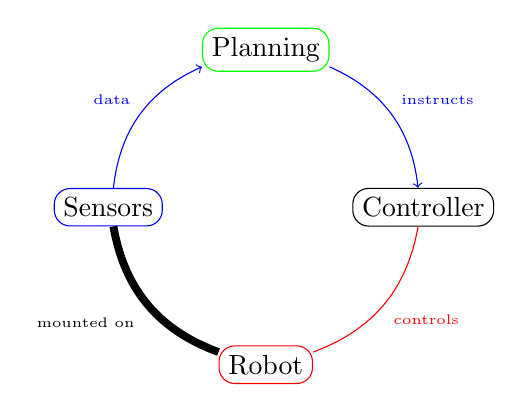
\begin{tikzpicture}[align=center]
            \node[actuator](robot) at (0,0) {Robot};
            \node[sensor](lidar) at (-2,2) {Sensors};
            \node[software](path) at (0,4) {Planning};
            \node[control](controller) at (2,2) {Controller};
      
            \draw[boldline] (robot) edge[bend left] node[below left]{\tiny mounted on} (lidar);
            \draw[rosline] (lidar) edge[bend left] node[above left]{\tiny data} (path);
            \draw[rosline] (path) edge[bend left] node[above right]{\tiny instructs} (controller);
            \draw[controlline] (controller) edge[bend left] node[below right]{\tiny controls} (robot);
         \end{tikzpicture}
      \end{column}

      \begin{column}{.5\textwidth}
         \begin{itemize}
            \item ROS uses nodes, topics and messages in a publisher subscriber like pattern
            \item \textbf{Glue} that holds everything together
            \item Asynchron and Real time capabilites
         \end{itemize}
      \end{column}
   \end{columns}
\end{frame}

\begin{frame}{ROS -- Example}
   \centering
   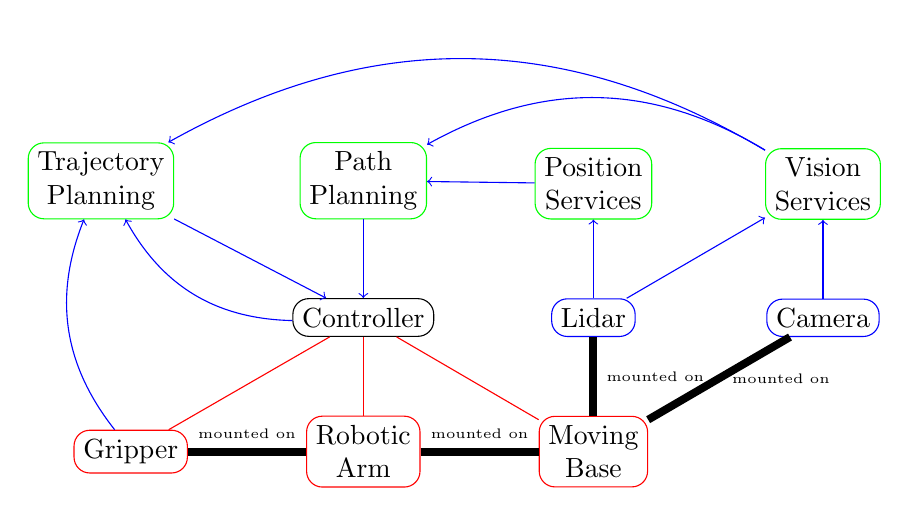
\begin{tikzpicture}[align=center, auto, node distance=1cm and 1.5cm] 
      \node[actuator](gripper) at (0,0) {Gripper};
      \node[actuator](arm) [right = of gripper] {Robotic\\ Arm};
      \node[actuator](base) [right = of arm] {Moving\\ Base};

      \node[sensor](lidar) [above = of base] {Lidar};
      \node[sensor](camera) [above right = of base] {Camera};

      \node[software](positioning) [above = of lidar] {Position\\ Services};
      \node[software](vision) [above = of camera] {Vision\\ Services};

      \node[control](controller) [above = of arm] {Controller};
      
      \node[software](path) [above = of controller] {Path\\ Planning};
      \node[software](trajectory) [above left = of controller] {Trajectory\\ Planning};


      \draw[boldline] (gripper) -- node[above]{\tiny mounted on} (arm) ;
      \draw[boldline] (arm) -- node[above]{\tiny mounted on} (base);
      \draw[boldline] (camera) -- node[right]{\tiny mounted on} (base);
      \draw[boldline] (lidar) -- node[right]{\tiny mounted on} (base);
      \draw[rosline] (lidar) -- (positioning);
      \draw[rosline] (lidar) -- (vision);
      \draw[rosline] (camera) -- (vision);

      \draw[controlline] (controller) -- (gripper);
      \draw[controlline] (controller) -- (arm);
      \draw[controlline] (controller) -- (base);

      \draw[rosline] (vision) edge[bend right] (path);
      \draw[rosline] (positioning) -- (path);

      \draw[rosline] (vision) edge[bend right] (trajectory);

      \draw[rosline] (controller) edge[bend left] (trajectory);
      
      \draw[rosline] (gripper) edge[bend left] (trajectory);

      \draw[rosline] (trajectory) -- (controller);
      \draw[rosline] (path) -- (controller);
   \end{tikzpicture}
\end{frame}


\begin{frame}{Gazebo}
   \begin{itemize}
      \item powerful tool used for simulationg robotic systems and enviroments
      \item 3D physic-based simulation platform
      \item Robots can be tested and developed before deploying
   \end{itemize}

   \begin{figure}
      \includegraphics[width=0.3\textwidth]{images/gazebo_logo.png}
   \end{figure}
\end{frame}

\begin{frame}{Gazebo -- Drawbacks}
   \begin{itemize}
      \item Physical accuracy and anomalies
      \item Stability of software
      \item Lack for complex enviroments and terrain
      \item Realism of Graphics
   \end{itemize}
   \begin{columns}[c]
      \begin{column}{.5\textwidth}         
         \begin{figure}
            \includegraphics{images/gazebo.png}
            \caption{https://gazebosim.org}
         \end{figure}
      \end{column}
      \begin{column}{.5\textwidth}  
         \begin{figure}
            \includegraphics{images/unreal_arisim.png}
            \caption{Unreal Engine AirSim \cite{shah2017airsim}}
         \end{figure}
      \end{column}
   \end{columns}
\end{frame}

\begin{frame}{Unreal Engine}
   Unreal Engine is a powerful and versatile game engine developed by Epic Games
   
   \begin{multicols}{2}
      \begin{itemize}
         \item advanced graphic capabilites
         \begin{itemize}
            \item realistic lighting
            \item advanced visual effects
            \item particle systems
            \item real time reflections
         \end{itemize}
         \item Cross Platform Support
         \item Extensive Toolset
         \begin{itemize}
            \item Terrain Editor
            \item Material Editor
         \end{itemize}
         \item Broad Community
         \begin{itemize}
            \item Unreal Marketplace
            \item Quixel Megascans
         \end{itemize}
      \end{itemize}
   \end{multicols}

   \begin{figure}
      \includegraphics[width=0.15\textwidth]{images/unreal_logo.png}
   \end{figure}
\end{frame}

\begin{frame}{Unreal Engine -- Game Engines for sumulations?}
   \begin{table}
      \begin{tabular}{>{\hfill}p{5cm} | c c}
         & Video Game & Simulation application \\ \hline
         Goal: Entertainment & \cmark & \xmark \\
         Goal: Learning & \xmark & \cmark \\
         Interoperable / Muliplayer & \cmark & \cmark \\
         Connected & \cmark & \cmark \\
         Visual and physical Realism & \cmark & \cmark \\
         Deployability & \cmark & \cmark \\
         Open & \cmark & \cmark \\
         Large open world & \cmark & \cmark \\
      \end{tabular}
   \end{table}
   \bigbreak
   The only difference between video games an simulation application is the goal
\end{frame}

\begin{frame}{Motivation}
   \textbf{Why do we need Simulation enviroments?}
   \begin{multicols}{2}
      \begin{itemize}
         \item Cost-Effective
         \item Safe
         \item Rapid Prototyping
         \item Testing
         \item Data generation
         \item \dots
      \end{itemize}
   \end{multicols}

   \begin{figure}
      \includegraphics[width=4cm]{images/fe-panda.jpg}
      \caption{https://www.mybotshop.de/FE-PANDA}
   \end{figure}

\end{frame}


\begin{frame}{Motivation --- Testing}
   Simulation allow for testing Cyber-Physical Systems without their direct deployment in the real world.
   \bigbreak
   Realistic physic engines are needed to generate valueable tests.
   \bigbreak
   With Simulations Cyber-Physical Systems can easily tested in an wide range of enviroments.
\end{frame}

\begin{frame}{Motivation --- Data generation}
   Data-driven algorithms play a crucial role especially in robotic vision problems.
   For training huge amounts of data needs to be gathered.
   \bigbreak
   Synthetic generation of data have become increasingly popular but require accurate replication of real world environments.
   
\end{frame}


\begin{frame}{Goal}
   \begin{columns}[c]
      \begin{column}{.5\textwidth}
         \begin{tikzpicture}
            \node[roundenode] (ros) at (0,0) {Roboter Operating System};
            \node[roundenode] (framework) [above = of ros] {Framework};
            \node[roundenode] (ue) [above = of framework] {Unreal Engine};
      
            \node [align=center] (file) [left = of framework] {\LARGE \faFileCodeO };
      
            \node [align=center] (log) [right = of framework, yshift=3mm] {\LARGE \faFileTextO };
            \node [align=center] (log) [right = of framework, yshift=-3mm] {\LARGE \faHddO };
            \node [align=center] (log) [right = of framework] {\phantom{\LARGE \faHddO}};
            
            \node [anchor=north west] at (0,1.1) {\tiny subscribe};
            \node [anchor=north east] at (0,1.1) {\tiny publish};
            \draw (ros) edge[auto shift] (ue);
            \draw (ue) edge[auto shift] (ros);
      
            \draw (file) -- node[above]{\tiny config} (framework);
            \draw (framework) -- node[above]{\tiny log} (log);
      
            \node[roundenode, fill=white] (framework) [above = of ros] {Framework};
      
            \draw[red,thick,dotted] ($(file.north west)+(-0.3,0.6)$)  rectangle ($(log.south east)+(0.3,-0.6)$);
         \end{tikzpicture}
      \end{column}
      \begin{column}{.5\textwidth}
         \begin{itemize}
            \item Unreal Engine Plugin
            \item Automatic simulations with Unreal Engine
            \item Configuration / Simulation-Description
            \item Interface for logging and data dumping
         \end{itemize}
      \end{column}
   \end{columns}
\end{frame}

\begin{frame}{Timetable}
   \newganttchartelement*{equalateralmilestone}{
      equalateralmilestone/.style={
         shape=diamond,
         draw,
         fill=black,
      },
      equalateralmilestone label font=\slshape,
      equalateralmilestone left shift=1.0,
      equalateralmilestone right shift=-1.0,
      }

   \begin{ganttchart}[
      expand chart=\linewidth,
      y unit chart=6mm,
      time slot format=little-endian,
      today=2.4.24,
      progress=today,
      hgrid,
      vgrid={*6{draw=none}, *1{dotted}}
   ]{1.3.24}{30.8.24}
      %labels
      \ganttset{calendar week text=\currentweek} % Overload the week text, display the week number (1, 2,, ...) instead of "Week <number>"
      \gantttitlecalendar{month=name}\\
      %tasks
      \ganttbar{Research}{1.3.24}{15.4.24}\\
      \ganttbar{ROS $\leftrightarrows$ UE}{1.04.24}{15.05.24}\\
      \ganttequalateralmilestone{Initial}{9.4.24}\\
      \ganttgroup{UE Plugin}{1.05.24}{1.08.24}\\
      \ganttbar{UE config}{1.05.24}{1.06.24}\\
      \ganttbar{UE model}{1.06.24}{1.07.24}\\
      \ganttbar{UE terrain}{1.07.24}{1.08.24}\\
      \ganttbar{Thesis}{15.6.24}{30.8.24}

   
   \end{ganttchart}

\end{frame}

%% to show a last slide similar to the title slide: information for the last page
\title{Thank you for your attention!}
\subtitle{Any questions?}
\author{}
\URL{}
\section{Thanks}


%% appendix of 'extra' slides
\appendix

\begin{frame}{References}
   \bibliographystyle{plain}
   \bibliography{refs}
\end{frame}

\begin{frame}{Gazebo IDE}
   
   \begin{columns}[c]
      \begin{column}{.5\textwidth}
         \begin{figure}
            \includegraphics{images/gazebo_ex1.png}
            \caption{Positioning and Path Planning}
         \end{figure}
      \end{column}
      \begin{column}{.5\textwidth}
         \begin{figure}
            \includegraphics{images/gazebo_ex2.jpeg}
            \caption{Drone Simulation}
         \end{figure}
      \end{column}
   \end{columns}
\end{frame}
\end{document}
